\title{Final Exam for Algebra-Based Physics-2: Electricity, Magnetism, and Modern Physics (PHYS135B-01)}
\author{Dr. Jordan Hanson - Whittier College Dept. of Physics and Astronomy}
\date{\today}
\documentclass[10pt]{article}
\usepackage[a4paper, total={18cm, 27cm}]{geometry}
\usepackage{outlines}
\usepackage[sfdefault]{FiraSans}
\usepackage{hyperref}
\usepackage{graphicx}
\begin{document}
\maketitle

\begin{enumerate}
\item \textbf{Electric charge and electric fields}
\begin{enumerate}
\begin{figure}[ht]
\centering
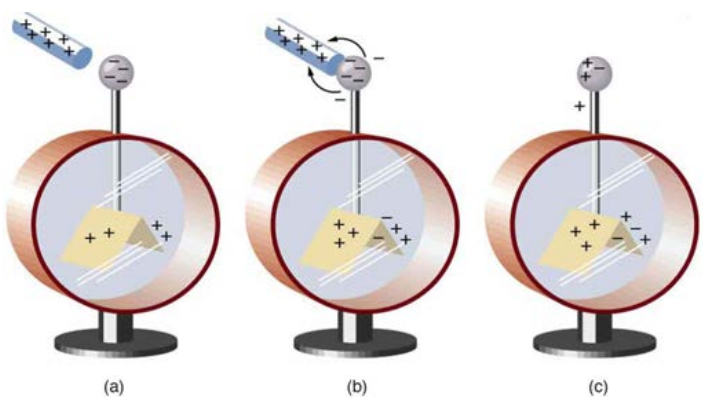
\includegraphics[width=0.35\textwidth]{figures/elec.png}
\caption{\label{fig:elec} Touching charge to an electroscope.  A glass rod with a positive net charge is moved near the ball.  Initially, the electroscope is electrically neutral.}
\end{figure}
\item In process (a)-(c) of Fig. \ref{fig:elec}, an electroscope gains a positive charge.  The gold leaves each have a net positive charge and therefore remain apart.  Suppose a charged particle like a cosmic ray passes between the leaves, and ionizes the air such that there is \textit{temporarily} a negative charge in the air between the plates.  What will happen?
\begin{itemize}
\item A: Nothing will happen.  The leaves will remain apart.
\item B: The angle between the leaves will decrease to a new value, and remain at that new value.
\item C: The angle between the leaves will decrease to a new value temporarily, and spring back to the old value.
\end{itemize}
\item Suppose one of the leaves in the electroscope in Fig. \ref{fig:elec} is hit by a cosmic ray, and the cosmic ray \textit{neutralizes it.}  What will happen?
\begin{itemize}
\item A: Nothing will happen.  The leaves will remain apart.
\item B: The angle between the leaves will decrease to a new value, and remain at that new value.
\item C: The angle between the leaves will decrease to a new value temporarily, and spring back to the old value.
\item D: The angle between the leaves will decrease to zero.
\end{itemize}
\begin{figure}[hb]
\centering
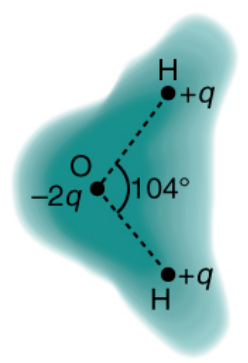
\includegraphics[width=0.12\textwidth]{figures/h20.png}
\caption{\label{fig:dipole} An illustration of the dipole moment of a water molecule.}
\end{figure}
\item The charge distribution of a water molecule is modeled in Fig. \ref{fig:dipole}.  Recall that the electric \textit{dipole moment} is $\vec{p} = q\vec{d}$, where $d$ is a vector pointing from $-q$ to $+q$.  There are two such vectors in the water molecule model in Fig. \ref{fig:dipole}.  In which direction does their sum point?  This is the net dipole moment.
\begin{itemize}
\item A: Up
\item B: Down
\item C: Left
\item D: Right
\end{itemize}
\item If the molecule is in an electric field in the plane of the page and pointing up, what will happen?
\begin{itemize}
\item A: It will remain stationary.
\item B: It will move up, but not spin.
\item C: It will spin clockwise.
\item D: It will spin counter-clockwise.
\end{itemize}
\item If the molecule is in an electric field in the plane of the page and pointing down, what will happen?
\begin{itemize}
\item A: It will remain stationary.
\item B: It will move down, but not spin.
\item C: It will spin clockwise.
\item D: It will spin counter-clockwise.
\end{itemize}
\end{enumerate}
\item \textbf{Electric potential and electric fields}
\begin{figure}[hb]
\centering
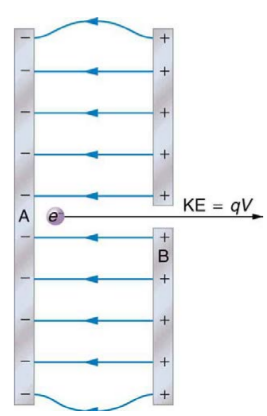
\includegraphics[width=0.2\textwidth]{figures/plate2.png}
\caption{\label{fig:plate2} An electron is accelerated through a potential $V$.}
\end{figure}
\begin{enumerate}
\item Suppose the voltage in Fig. \ref{fig:plate2} is 1 MV, and the particle has a charge equal to \textit{three electrons}.  The final energy of the particle is
\begin{itemize}
\item A: 1 keV
\item B: 3 keV
\item C: 1 MeV
\item D: 3 MeV
\end{itemize}
\item Suppose the charge of the particle in Fig. \ref{fig:plate2} is decreased by a factor of three.  The final energy
\begin{itemize}
\item A: Increases by a factor of 3
\item B: Increases by a factor of $\sqrt{3}$
\item C: Decreases by a factor of 3
\item D: Decreases by a factor of $\sqrt{3}$
\end{itemize}
\item Recall that the relationship between the voltage, electric field, and separation in a capacitor is $V = E d$.  What is the electric field inside a capacitor with separation $1$ mm, and is charged at $3.3$ V?
\begin{itemize}
\item A: 330 V/m
\item B: 3.3 mV/m
\item C: 33 V/m
\item D: 3.3 kV/m
\end{itemize}
\item Graph the voltage versus separation for the capacitor in the previous problem, and label the axes with approprate units.  Indicate the x and y-intercepts and their corresponding numerical values. \\ \vspace{3cm}
\item The capacitance of a parallel plate capacitor is $C = \epsilon_0 A/d$, where $A$ is the area of the plates, $d$ is the separation between the plates, and $\epsilon_0 = 8.85 \times 10^{-12}$ N$^{-1}$ C$^2$ m$^{-2}$.  What is the capacitance of a capacitor with an area of 2 mm$^2$ and a separation of 0.1 mm? \\ \vspace{2cm}
\end{enumerate}
\item \textbf{Electric current, resistance, and Ohm's law}
\begin{enumerate}
\item Recall that Ohm's law states that $V = iR$, and that resistors in series add, while resistors in parallel add in reciprocal.  Find the total current from the battery in the circuit drawn in Fig. \ref{fig:circuit}.
\begin{figure}[hb]
\centering
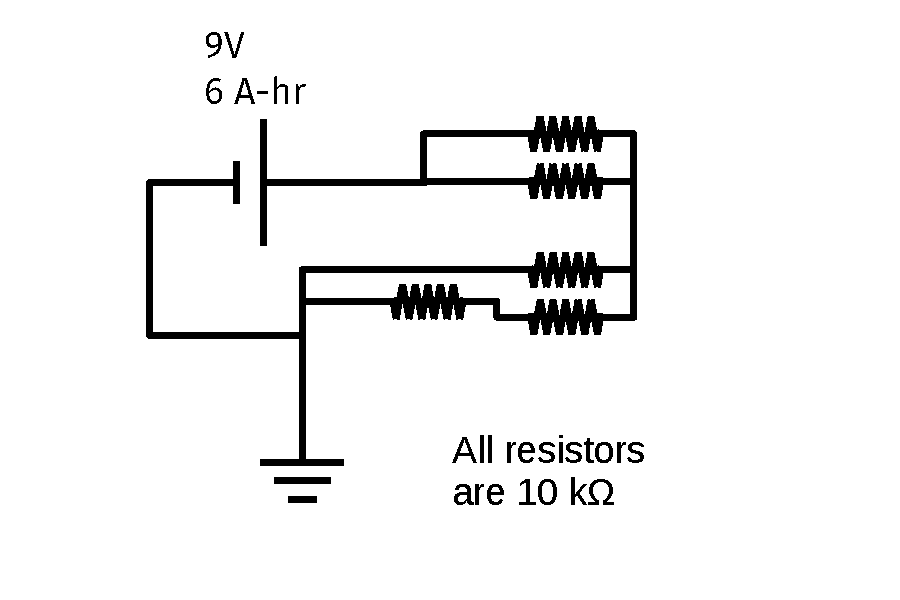
\includegraphics[width=0.5\textwidth]{figures/circuitExample2.pdf}
\caption{\label{fig:circuit} A DC circuit with a battery voltage of 9V and five identical resistors.}
\end{figure}
\item How long before the charge in the battery is drained in the circuit in Fig. \ref{fig:circuit}? \\ \vspace{3cm}
%\begin{figure}
%\centering
%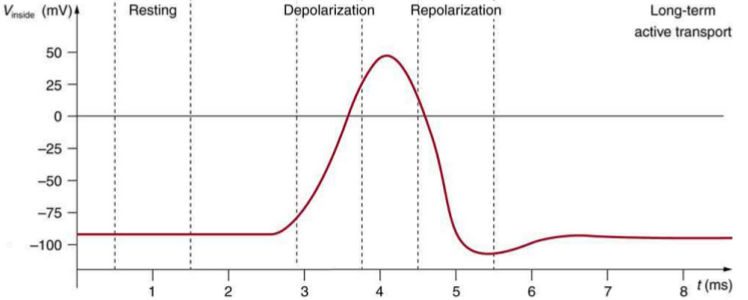
\includegraphics[width=0.4\textwidth]{figures/action.png}
%\caption{\label{fig:action} The voltage versus time of a nerve action pulse.}
%\end{figure}
%\item How are the four stages of the voltage pulse in Fig. \ref{fig:action} created in the human body? \\ \vspace{4cm}
\end{enumerate}
\item \textbf{Magnetism}
\begin{enumerate}
\begin{figure}
\centering
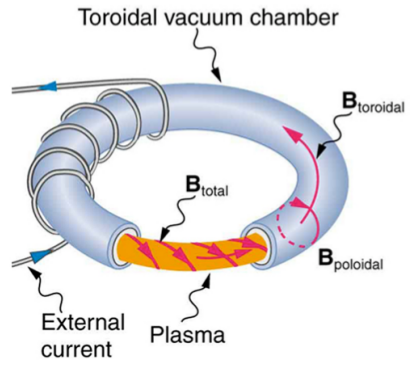
\includegraphics[width=0.25\textwidth]{figures/tok.png}
\caption{\label{fig:tok} The basic premise of a tokamak, containing plasma for fusion reactions.}
\end{figure}
\item The toroidal magnetic field in the tokamak fusion reactor in Fig. \ref{fig:tok} is created by the external current.  The plasma is hot ionized gas, and the \textit{poloidal} magnetic field is created by it.  If the direction of the current were reversed, in which direction would the toroidal magnetic field point?
\begin{itemize}
\item A: Counter-clockwise
\item B: Clockwise
\item C: Towards the center of the circle
\item D: Away from the center of the circle
\end{itemize}
\item A particular \textit{proton} has a velocity component perpendicular to the toroidal field and parallel to the poloidal field.  Describe its motion in words. \\ \vspace{2cm}
\item A particular \textit{electron} has a velocity component perpendicular to the toroidal field and parallel to the poloidal field.  Describe its motion in words. \\ \vspace{2cm}
\item The velocity of a fluid flowing through the line in Fig. \ref{fig:hall} is being measured using the Hall effect.  If the magnetic field is $10$ gauss ($10^{-3}$ T), the line has $l = 2$ cm, and $v = 20$ m/s, what is the Hall voltage?  \\ \vspace{2cm}
\begin{figure}[hb]
\centering
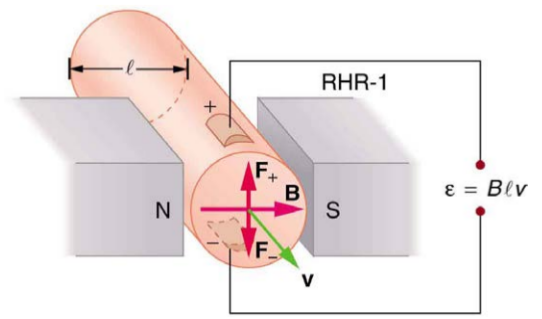
\includegraphics[width=0.3\textwidth]{figures/hall.png}
\caption{\label{fig:hall} A hall voltage measurement of the velocity of a fluid.}
\end{figure}
\end{enumerate}
\item \textbf{Electromagnetic waves}
\begin{enumerate}
\item Recall that $c = f\lambda$.  Using the speed of light ($c = 3.0 \times 10^8$ m/s), convert each of the following frequencies to their corresponding wavelengths:
\begin{itemize}
\item 1 kHz
\item 100 kHz
\item 1 MHz
\end{itemize}
\item Recall that $c = f\lambda$ is modified to $c/n = f\lambda$ when an electromagnetic wave is traveling in a dielectric material, where $n$ is the index of refraction.  Suppose we record a radio wave traveling through a block of a substance that is 1000 m long, and the wave travels for 7300 ns from the start to the end of the block.  What is the index of refraction $n$? \\ \vspace{2cm}
\end{enumerate}
\end{enumerate}
\end{document}